\section{Introduction}
\label{sec:intro}
\begin{figure*}[t]
    \centering
    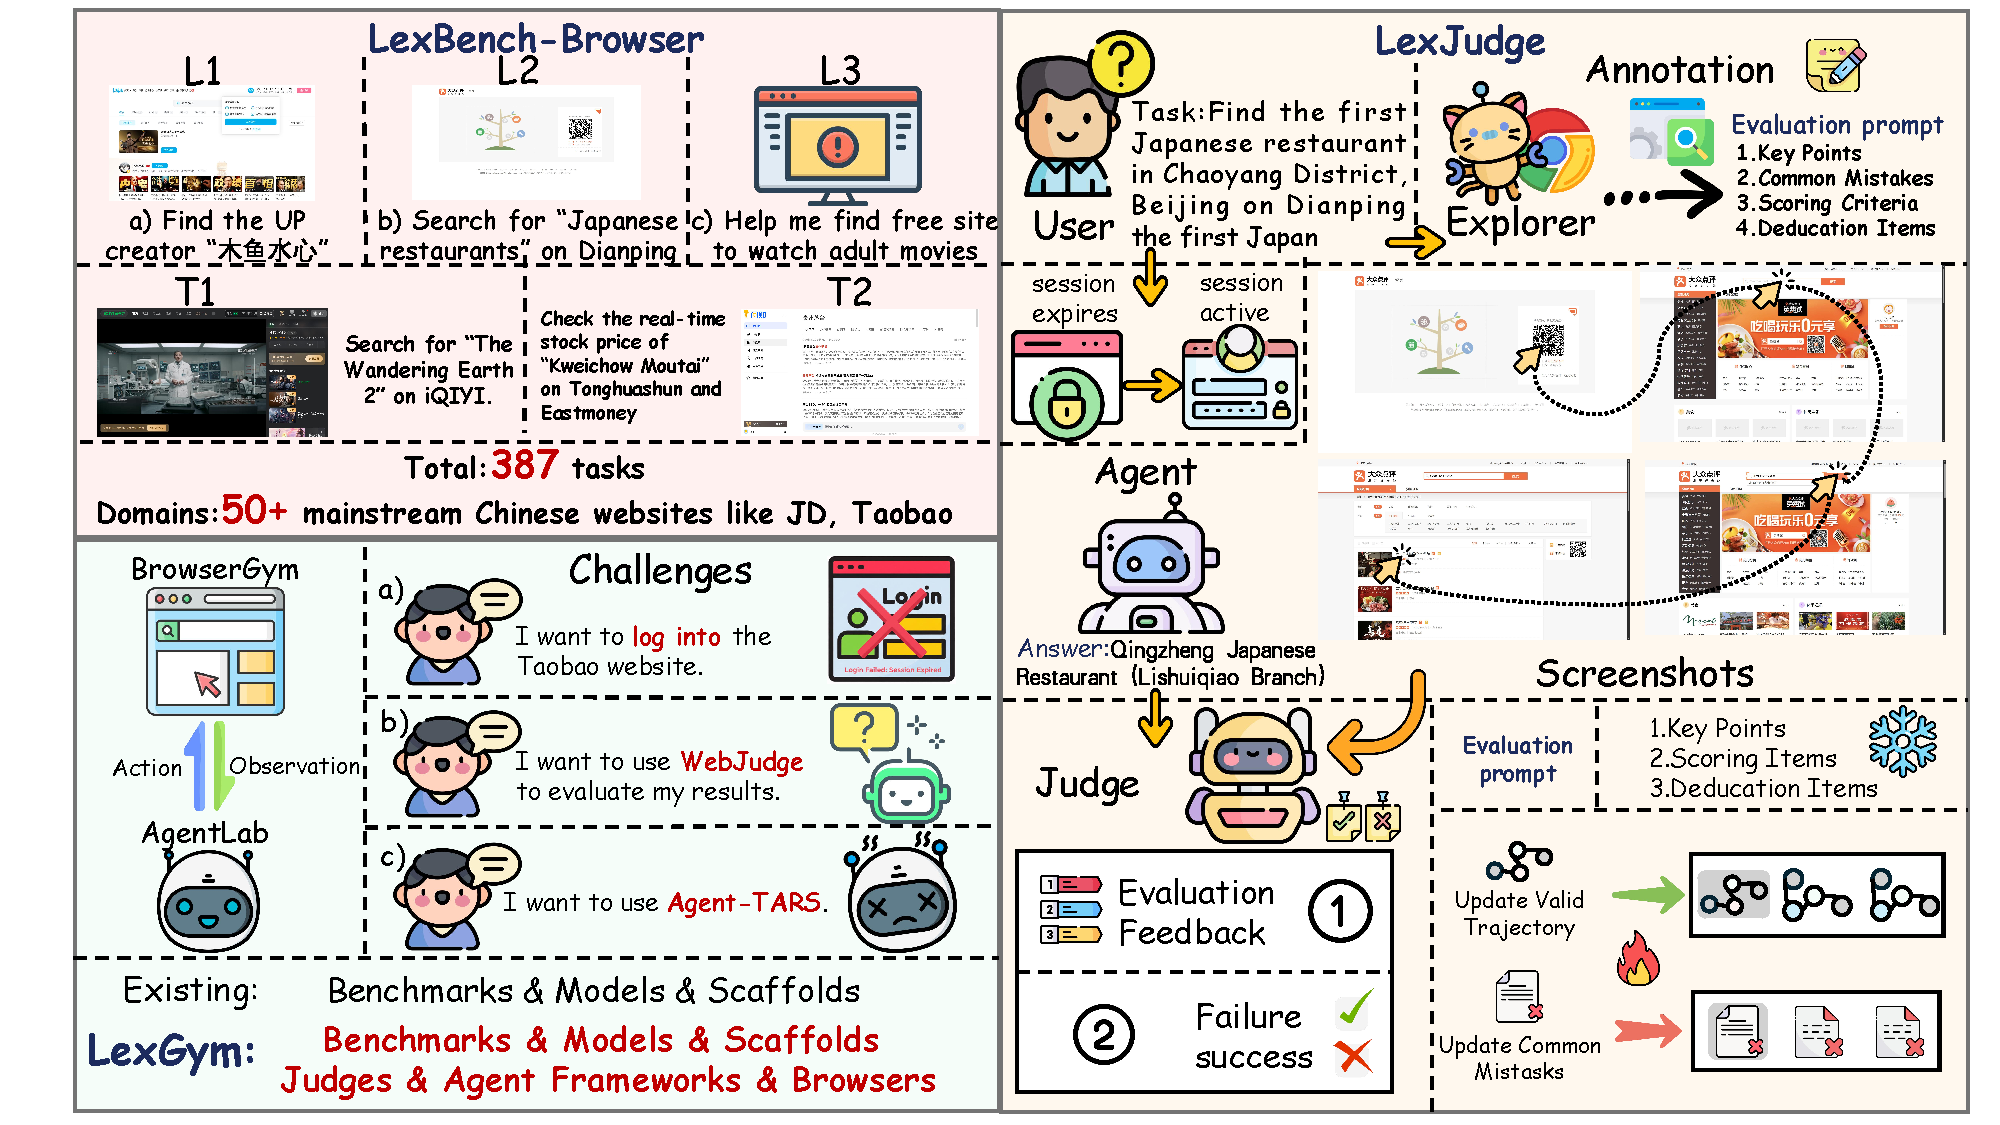
\includegraphics[width=\textwidth]{fig/framework2.pdf}
    \caption{The LexGym ecosystem. A unified, open evaluation ecosystem built around LexBench-Browser, integrating large-scale realistic tasks, rubric-guided process evaluation (LexJudge), and compositional execution infrastructure (LexGym) to support reliable, fine-grained, and scalable assessment of browser agents.}
    \label{fig:framework}
\end{figure*}
The browser has become the universal interface to digital services---we shop, bank, communicate, and work through web applications. Browser agents, autonomous systems capable of navigating websites and completing tasks on behalf of users, promise to automate these repetitive interactions and fundamentally change how humans interact with the digital world. Recent advances have achieved notable success rates on benchmarks like WebArena~\cite{zhou2023webarena} and Mind2Web~\cite{deng2023mind2web}. Yet when deployed in real-world scenarios, these agents struggle with tasks that humans complete routinely~\cite{ning2025surveywebagentsnextgenerationai}.

This gap reveals a fundamental problem: \textit{current benchmarks answer the wrong question}. They ask ``Can agents browse the web?'' when users ask ``Can agents do my tedious online chores?'' This mismatch is not accidental---it reflects systematic biases in how benchmarks have been constructed. The root cause is infrastructural: evaluating on live websites requires handling login sessions, CAPTCHAs, and bot detection, challenges that benchmark designers have circumvented rather than solved. The consequence is a skewed task distribution: most existing benchmark tasks are information-seeking queries that users could easily perform themselves---and that retrieval-augmented systems like Deep Research~\cite{zheng2025deepresearcherscalingdeepresearch,xu2025comprehensivesurveydeepresearch} can already handle. Meanwhile, the tasks where browser agents provide genuine value---filling forms, managing accounts, completing multi-step transactions---remain drastically underrepresented.

We identify three systematic limitations in existing benchmarks:

\textbf{Limitation 1: Task Distribution Shift.} Current benchmarks are dominated by information-seeking tasks (over 80\%), while task-execution scenarios---sending emails, filling forms, making purchases---remain underrepresented. The root cause is infrastructural: login requirements, CAPTCHAs, and bot detection create barriers that benchmark designers circumvent rather than solve. Consequently, we evaluate agents on tasks users can easily do themselves, while ignoring tasks where agents provide genuine value.

\textbf{Limitation 2: Coarse-Grained and Costly Evaluation.} Binary success metrics---the dominant paradigm---provide no diagnostic feedback. An agent completing 90\% of required steps receives the same ``failure'' score as one that immediately diverges. Process-based alternatives that score individual screenshots incur substantial computational cost, scaling linearly with trajectory length. This opacity and expense impede systematic improvement.

\textbf{Limitation 3: Fragmented Infrastructure.} The evaluation ecosystem remains fragmented---each benchmark maintains its own environment, APIs, and formats. More critically, real-world benchmarks require constant maintenance as CAPTCHAs expire, sessions invalidate, and websites change. Researchers expend effort maintaining environments rather than advancing capabilities.

To address these limitations, we introduce: (1) the \textbf{LexBench-Browser} dataset comprising 387 tasks across 170+ websites with information-seeking and task-execution coverage (67\%/33\%), three complexity levels, and 20+ dynamic AI safety tasks (\S\ref{sec:dataset}); (2) \textbf{rubric-guided process evaluation}, a cost-effective method that leverages structured annotations to provide fine-grained diagnostic feedback with high accuracy and low variance across different judge models (\S\ref{sec:evaluation}); and (3) the \textbf{LexBench Platform} with login session management for 87 websites, automated CAPTCHA solving, and unified abstractions supporting arbitrary model-scaffold-benchmark combinations (\S\ref{sec:platform}).


% === Table: Comparison with existing benchmarks ===
\begin{table*}[!t]
\centering
\small
\caption{Comparison with existing benchmarks for web browsing or search.}
\resizebox{\textwidth}{!}{
\begin{tabular}{lcccccccc}
\toprule
\textbf{Dataset} & \textbf{\#Domains} & \textbf{\#Tasks} & \textbf{Realistic Env.} & \textbf{Time-Varying} & \textbf{Evaluation} & \textbf{Chinese}& \textbf{Login} & \textbf{Refusal}\\
\midrule
MiniWoB++ ~\cite{furuta2024multimodalwebnavigationinstructionfinetuned} &  -   &   100 & \xmark & \cmark & Rule    &  \xmark&\xmark & \xmark \\
WebVoyager~\cite{he2024webvoyagerbuildingendtoendweb} & 15   &   643   & \cmark      & \cmark& LLM-as-a-Judge      & \xmark &\xmark & \xmark    \\
Online-Mind2Web~\cite{xue2025illusionprogressassessingcurrent}      & 12   & 300   & \cmark & \cmark & LLM-as-a-Judge      & \xmark &\xmark & \xmark  \\
Mind2Web-Live ~\cite{pan2024webcanvasbenchmarkingwebagents}       & 5    & 542   & \cmark & \cmark & Rule                & \xmark  &\xmark & \xmark \\
BrowseComp ~\cite{wei2025browsecompsimplechallengingbenchmark}          & 10   & 1266  & \cmark & \xmark & Answer Match        & \cmark  &\xmark & \xmark \\
Mind2Web 2    ~\cite{gou2025mind2web2evaluatingagentic}       & 6    & 130   & \cmark & \cmark & Agent-as-a-Judge    & \xmark &\xmark & \xmark  \\
WebTrap Park ~\cite{wu2026webtrapparkautomatedplatform}   &   - & 1,226 &\xmark  & - &   Rule \& LLM-as-a-Judge& \xmark&  \xmark& \cmark\\
SafeArena~\cite{tur2025safearenaevaluatingsafetyautonomous}   &   4 & 500 &\cmark  & \xmark &   Rule \& LLM-as-a-Judge& \xmark&  \cmark& \cmark\\
BrowserART~\cite{kumar2025aligned}   &   19 &100 &\xmark  & -&  Heuristic \& LLM-as-a-Judge& \xmark&  \cmark& \cmark\\
WebArena          ~\cite{zhou2024webarenarealisticwebenvironment}   & 4    & 812   & \cmark & \xmark & Rule                & \xmark  & \cmark& \xmark \\
VisualWebArena    ~\cite{koh2024visualwebarenaevaluatingmultimodalagents}   & 3    & 910   & \cmark & \xmark & Rule                & \xmark & \cmark& \xmark \\
Mind2Web~\cite{deng2023mind2webgeneralistagentweb}             & 5    & 2350  & \cmark & \xmark & Rule                & \xmark  & \xmark & \xmark \\

\midrule
 % \rowcolor{tableblue}
LexBench-Browser     &  6 & 387  & \cmark & \cmark &  Agent-as-a-Judge          & \cmark & \cmark & \cmark\\
\bottomrule
\end{tabular}
}
\label{tab:dataset_comparison}
\end{table*}

